\documentclass[Afour,sagev,times]{sagej}

% SAGE template derived from manuscript_template.zip supplied with this project.
% Add the `doublespace` class option before journal submission if requested.
\usepackage{url}
\usepackage[colorlinks=true,linkcolor=black,citecolor=black,urlcolor=blue]{hyperref}
\usepackage{graphicx}
\usepackage{amsmath}
\usepackage{enumitem}
\usepackage{booktabs}
\usepackage{tabularx}
\usepackage{array}
\usepackage{xcolor}
\usepackage{placeins}
\usepackage{float}

% Keep float-only pages aligned with the manuscript text block rather than
% vertically centering sparse tables or figures.
\makeatletter
\setlength{\@fptop}{0pt}
\setlength{\@dblfptop}{0pt}
\makeatother

\graphicspath{{generated/figures/}}
\newcolumntype{Y}{>{\raggedright\arraybackslash}X}

\begin{document}
\raggedbottom

\runninghead{Ghorbannia et al.}
\title{Conceptual Clarification of Digital Patient Frameworks, Methodological Approaches, and Infrastructural Gaps: Evidence from a Systematic Meta-Review}

\author{Arash Ghorbannia\affilnum{1}, Mark Scerbo\affilnum{1}, Megan Witherow\affilnum{1}, Faryaneh Poursardar\affilnum{1}, April Pace\affilnum{1}, Taryn Couper\affilnum{1}, Jae H. Lee\affilnum{1}, Ginger Watson\affilnum{1}, Eric Weisel\affilnum{1} and Charles Combs\affilnum{1}}

\affiliation{\affilnum{1}Old Dominion University, Norfolk, VA, USA; National Center for Collaboration in Medical Modeling and Simulation, Old Dominion University, Norfolk, VA, USA. Author-specific affiliations should be confirmed before submission.}

\corrauth{Arash Ghorbannia, Old Dominion University, Norfolk, VA, USA.}
\email{Corresponding email to be confirmed before submission.}

\begin{abstract}
\textbf{Background:} Digital patient frameworks are expanding rapidly, but terms such as digital twin, virtual patient, in silico patient, and synthetic patient are used inconsistently.
\textbf{Objective:} To synthesize how recent healthcare reviews define, construct, validate, and operationalize the digital patient spectrum.
\textbf{Methods:} Following the PROSPERO protocol, we searched health, engineering, and grey-literature sources for English-language reviews published from 2020 onward and extracted review-level data with a CADIMA-aligned form. A version-controlled pipeline applies documented record-level classification rules and regenerates all manuscript tables and figures.
\textbf{Results:} The reproducible analytic set contains 64 coded records representing 62 unique normalized review titles. Applications span multiple clinical domains, while validation, reproducibility, interoperability, governance, and clinical maturity remain unevenly reported.

\textbf{Conclusions:} The field is conceptually active but infrastructurally immature. Translation will require clearer taxonomy, stronger validation standards, interoperable data architecture, and governance models for clinically deployable patient digital twins.

\end{abstract}

\keywords{digital patient, digital twin, virtual patient, in silico patient, systematic review, meta-review, reproducibility}

\maketitle

\section{Introduction}

Digital patient frameworks promise computable representations of human biology that can support prediction, personalization, simulation, education, and clinical decision-making. The terminology is broad: healthcare reviews use labels including digital twin, patient digital twin, virtual patient, in silico patient, synthetic patient, digital avatar, and digital patient, often with overlapping but non-identical meanings.

This conceptual spread matters because different terms imply different technical commitments. A virtual or in silico patient may be static, archetype-based, or population-level, whereas the term digital twin often implies tighter patient-specific and temporal coupling. Without clearer boundaries, claims about maturity, validation, and clinical readiness remain difficult to compare.

Existing standards and guidance address complementary parts of this problem rather than a single end-to-end framework for digital patients. Cross-domain consensus characterizes a digital twin by dynamic updating, predictive capability, decision relevance, and bidirectional interaction with its physical counterpart, while regulatory credibility frameworks make the evidentiary burden dependent on a defined context of use and model risk.\cite{nasem2024digitaltwins,fda2023credibility,asme2018vv40} Construct identity should therefore be distinguished from fitness for a clinical purpose.

Guided by the PROSPERO protocol, this meta-review addresses six prespecified review questions: conceptual framing; construction and modeling frameworks; validation and fidelity; the application spectrum and functional roles; barriers and infrastructural gaps; and future directions and standardization priorities. The data-extraction strategy is viewpoint-driven rather than purely bibliographic. Each coded field populates a specific interpretive layer: study characteristics define the evidence base; terminology clarifies conceptual boundaries; hierarchy, data coupling, and temporality locate constructs on the digital-patient spectrum; modeling inputs and outputs describe the computational pipeline; validation fields address credibility and clinical readiness; application fields define the use-case landscape; and barrier and future-direction fields inform an implementation roadmap.

The objective of this manuscript is to clarify how digital patient constructs are defined, built, validated, and applied across recent healthcare review literature, while making the descriptive synthesis fully reproducible from the accompanying extraction workbook.

\section{Methods}

\subsection{Design, registration, and reporting}

We conducted a systematic overview of reviews (meta-review) in accordance with a protocol prospectively registered in the International Prospective Register of Systematic Reviews (PROSPERO). An editable summary of the prespecified protocol is provided in Supplementary Appendix S1. Reporting was guided by PRISMA 2020 and the overview-specific PRIOR statement.\cite{page2021prisma,gates2022prior}

% AUTHOR ACTION: Insert the public PROSPERO CRD number and official record URL before submission.

\subsection{Information sources and search strategy}

We searched Web of Science, PubMed, IEEE Xplore, and Google Scholar. Supplementary searches covered reference lists of included reviews and the preprint servers TechRxiv, arXiv, bioRxiv, engrXiv, and medRxiv. Database-specific strategies combined controlled vocabulary, where available, and free-text terms for digital twins and adjacent digital patient constructs, human health and healthcare, and review methodology. Searches were limited to English-language reports published from 2020 onward. Initial searches were conducted in October 2025, with an updated search specified before final manuscript submission. The complete conceptual search strategy is reproduced in Supplementary Appendix S1.

% AUTHOR ACTION: Report the exact last-search date and complete database-specific strategies before submission.

\subsection{Eligibility criteria}

Eligible reports were systematic reviews, meta-reviews, umbrella reviews, scoping reviews, or structured narrative reviews that explicitly examined at least one generic or patient-specific digital model applied to human health. The model had to represent human physiology, biomechanics, or another biological process and address at least one review domain: conceptualization, construction, validation, application, or methodological evaluation. Eligible models could operate from the subcellular level through whole-body or in silico population levels.

We excluded primary studies without a structured review methodology; editorials, perspectives, commentaries, and conference abstracts without sufficient methodological detail; non-English reports; animal-only or non-biological models; and reviews limited to hospitals, logistics, infrastructure, communication systems, or medical devices without a patient-level modeling component. Reviews focused exclusively on behavioral or educational simulations without a physiological, biomechanical, or biological patient representation were also excluded.

\subsection{Study selection and inconsistency resolution}

Records were managed and screened in CADIMA. At title and abstract screening, each record was assessed independently by two reviewers using three questions: whether the report was a review with structured methodology, whether it addressed digital twins or any conceptually related term identified within the broader digital patient spectrum (such as virtual patient, in silico patient, or synthetic patient), and whether it concerned human health or healthcare. Responses were recorded as Yes, Unclear, or No. A record progressed to full-text review when there was no agreed No on any core criterion.

CADIMA-flagged discrepancies were handled using the prespecified adjudication procedure reproduced in Supplementary Appendix S2. Discrepancies that could not change the inclusion decision were verified and finalized by the review coordinator acting as a third reviewer. Discrepancies that could change eligibility were discussed by the two reviewers, with each providing a brief rationale; unresolved uncertainty favored inclusion, and the coordinator made the final decision when consensus was not reached. Full-text reports were assessed against the complete eligibility criteria using the entire report, and exclusion reasons were recorded for the study-flow diagram. Search and selection results are reported using PRISMA 2020 and PRIOR conventions.\cite{page2021prisma,gates2022prior}

% AUTHOR ACTION: The available protocol and workbooks do not record how many reviewers independently assessed full texts. Confirm and report that number before submission.

\subsection{Data extraction}

Data were extracted in CADIMA using a standardized form mapped a priori to the six review questions. The form was piloted on a subset of included reviews and refined before full extraction; one reviewer completed each extraction and a second reviewer verified the entry for accuracy. Bibliographic and administrative data were collected for every review, while question-specific fields addressed conceptual framing (RQ1), construction and modeling (RQ2), validation and fidelity (RQ3), application domains and functional roles (RQ4), barriers and infrastructural gaps (RQ5), and future research and standardization priorities (RQ6). The complete field groups, extraction guidance, and mapping to the review questions are provided in Supplementary Table~\ref{tab:extraction-framework}. Because this was an overview of reviews, the form also recorded whether each review assessed methodological quality or risk of bias in its included primary studies, which tool or criteria were used, and whether those judgments informed the review's synthesis or interpretation.

\subsection{Methodological quality and risk of bias}

The prespecified appraisal framework treated methodological quality and risk of bias as related but distinct constructs. AMSTAR~2 was selected for applicable systematic reviews of healthcare evidence, and SANRA for structured narrative reviews.\cite{shea2017amstar2,baethge2019sanra} Review-level bias concerns were organized around the four ROBIS process domains: study eligibility criteria, identification and selection of studies, data collection and study appraisal, and synthesis and findings.\cite{whiting2016robis} The CADIMA appraisal further considered uncritical validation or fidelity claims, limited generalizability, implementation barriers, and incomplete reporting of funding or conflicts of interest. Each applicable concern was to be recorded as high concern, some concern or unclear, or low concern. Appraisal judgments were not intended as automatic exclusion criteria; they were intended to contextualize the strength, consistency, and limitations of the narrative synthesis.

% AUTHOR ACTION: Complete and independently verify the appraisal fields before reporting appraisal results; the current workbook contains missing and non-standardized entries.

\subsection{Synthesis and reproducible analysis}

Synthesis was narrative and descriptive; no quantitative pooling was planned because the included reviews differed in scope, terminology, model architecture, and reported outcomes. Prespecified comparisons considered generic or archetype-based versus patient-specific models, static versus dynamic or continuously coupled models, and educational versus clinical decision-support applications.

All transformations from the extraction workbook to manuscript tables and figures were scripted in Python. Predefined, case-insensitive lexical rules were applied only to prespecified extraction fields; common null and negation phrases were removed before classification, each theme was counted at most once per review, and reviews could contribute to multiple non-mutually-exclusive categories. When a review described multiple biological levels, the highest reported level was used only for the hierarchy visualization. Automated checks evaluated required fields, duplicate normalized titles, publication-year conflicts, missingness, output completeness, and study-flow arithmetic. Source data were read without modification, and derived tables, figures, plotting data, and quality-control reports were written separately. Analysis code, classification rules, and derived outputs are available in the public reproducibility repository described in the Data and code availability section.

\section{Results}

\subsection{Evidence base and study selection}

The current workbook contained 64 coded review records representing 62 unique normalized titles. Publication years were 2025 (28); 2024 (21); 2023 (9); 2022 (6). The most frequently matched domains were Cardiovascular (32); Oncology (25); Surgery / orthopedics / dentistry (24); Neurology / neuroscience (18); Diabetes / endocrine (17); the leading function categories were Treatment / therapy planning (56); Prediction / prognosis / risk (49); Diagnosis / detection (46); Education / training (19); Personalized care (9). The most frequently matched barrier groups were Privacy / security / governance (51); Ethical / legal / regulatory (51); Computing / scalability / resources (51); Interoperability / standards (49). Counts are record-level, rule-based, and non-mutually exclusive.


The evidence-base characteristics are summarized in Table~\ref{tab:characteristics}. Figure~\ref{fig:prisma} reports the project selection counts. Automated arithmetic checking identified a five-record discrepancy between the reported full-text exclusions and included studies; the source values are retained pending reconciliation.

\begin{figure}[H]
    \centering
    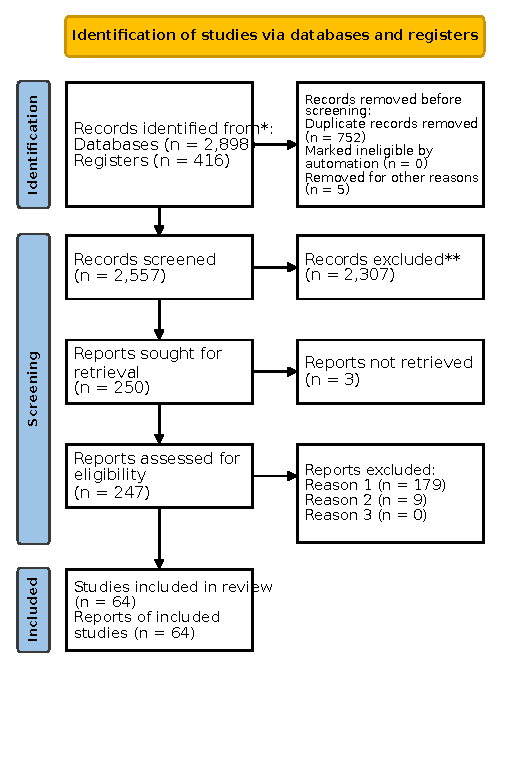
\includegraphics[width=\columnwidth]{fig1_prisma_single_portrait.pdf}
    \caption{PRISMA 2020 flow of records and reports. Source counts are retained pending reconciliation of the full-text arithmetic.}
    \label{fig:prisma}
\end{figure}

\begin{table*}[htbp]
\centering
\small
\caption{Characteristics of the included review evidence base.}
\label{tab:characteristics}
\begin{tabularx}{\textwidth}{@{}>{\raggedright\arraybackslash}p{0.20\textwidth}YY@{}}
\toprule
\textbf{Dimension} & \textbf{Current extracted signal} & \textbf{Interpretive use} \\
\midrule
Evidence base & 64 coded rows; 62 unique normalized titles; 2 duplicate-title rows. & Defines the analytic set and makes title-level duplicate reconciliation explicit. \\
Publication years & 2022: 6; 2023: 9; 2024: 21; 2025: 28; missing: 0. & Shows the temporal distribution using the canonical publication-year field with documented fallback. \\
Protocol scope & English-language reviews from 2020 onward addressing patient-linked physiological, biomechanical, biological, or adjacent computational models. & Keeps eligibility interpretation tied to the PROSPERO protocol. \\
Dominant domains & Cardiovascular (32); Oncology (25); Surgery / orthopedics / dentistry (24); Neurology / neuroscience (18); Diabetes / endocrine (17); General / multisystem (15) & Provides the empirical basis for the application landscape. \\
Quality context & Quality-appraisal and reproducibility fields are heterogeneous and incompletely populated. & Supports descriptive synthesis and cautious interpretation rather than pooled certainty claims. \\
\bottomrule
\end{tabularx}
\end{table*}


\subsection{Conceptual definitions and the digital patient spectrum}

The included reviews used digital twin terminology alongside patient digital twin, human digital twin, virtual patient, in silico patient or trial, digital patient, synthetic patient, and adjacent constructs. Patient specificity, biological hierarchy, temporal updating, and coupling direction varied independently, supporting a multidimensional spectrum rather than a single lexical definition (Table~\ref{tab:concepts}; Figure~\ref{fig:spectrum}).

\begin{table*}[htbp]
\centering
\small
\caption{Conceptual definitions and terminology across the digital patient spectrum.}
\label{tab:concepts}
\begin{tabularx}{\textwidth}{@{}>{\raggedright\arraybackslash}p{0.20\textwidth}YY@{}}
\toprule
\textbf{Conceptual dimension} & \textbf{Current extracted signal} & \textbf{Interpretive use} \\
\midrule
Primary terminology & Digital twin (47); Virtual patient (5); Human digital twin (5); Patient digital twin (4); In silico patient / trial (3) & Shows the distribution of the first identifiable primary construct per review record. \\
Patient specificity & Patient-specific/individualized (56); generic/population/archetype (28). & Separates individualized models from population-level or archetypal constructs; categories may overlap. \\
Temporal orientation & Dynamic/continuous (54); explicitly static (15). & Tests whether digital twin terminology is accompanied by longitudinal updating. \\
Data coupling & Bidirectional (33); one-way (39). & Distinguishes model-, shadow-, and twin-like coupling claims. \\
Hierarchy & Hierarchy levels are converted to an ordinal cell-to-system-of-systems scale for Figure 2; multi-level entries use the highest coded level. & Makes the spectrum plot reproducible while preserving the row-level source text. \\
\bottomrule
\end{tabularx}
\end{table*}


\begin{figure*}[!tbp]
    \centering
    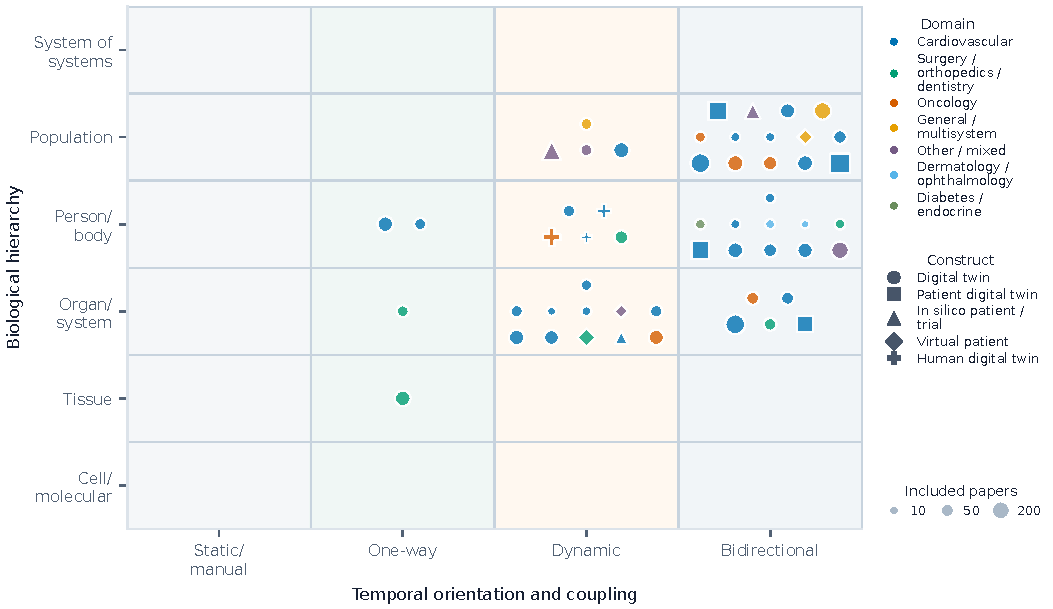
\includegraphics[width=0.96\textwidth]{fig2_spectrum_double_landscape.pdf}
    \caption{Digital patient spectrum. Records sharing a hierarchy--coupling category are deterministically spread within that cell to reduce overlap. Color denotes healthcare domain, marker shape denotes the primary construct, and marker area denotes the reported number of included papers.}
    \label{fig:spectrum}
\end{figure*}

\subsection{Modeling and computational pipeline}

Construction approaches were multimodal and heterogeneous. The extraction framework distinguishes data inputs, model families, personalization and coupling, named interoperability standards, computing infrastructure, and reported clinical or research outputs (Table~\ref{tab:pipeline}; Figure~\ref{fig:pipeline}).

\input{generated/tables/table3_pipeline}

\begin{figure*}[!tbp]
    \centering
    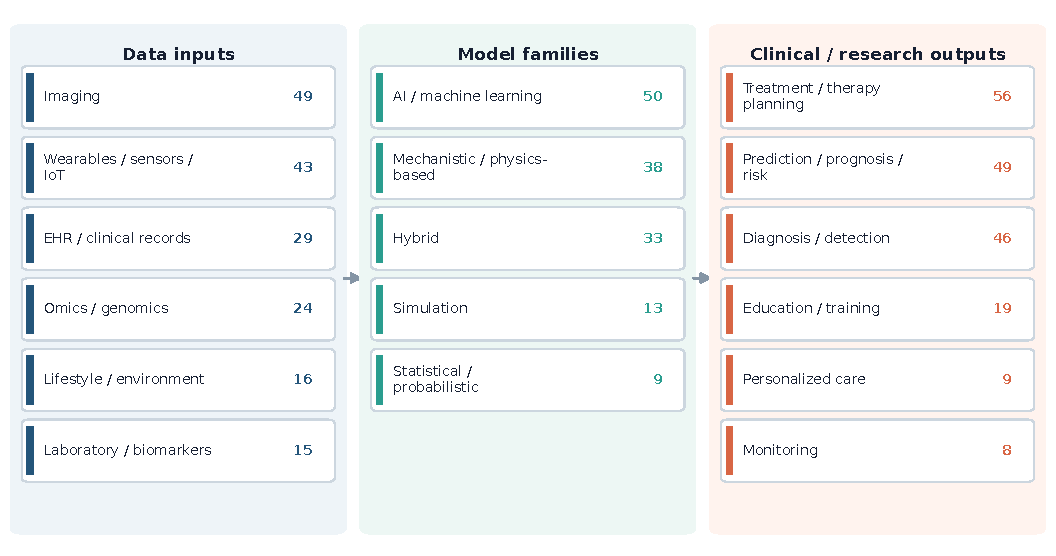
\includegraphics[width=0.96\textwidth]{fig3_pipeline_double_landscape.pdf}
    \caption{Computational pipeline across included reviews. Values are record-level mentions and categories are not mutually exclusive.}
    \label{fig:pipeline}
\end{figure*}

\subsection{Validation, fidelity, and clinical maturity}

Validation reporting ranged from conceptual discussion to empirical patient-data evaluation, simulation or benchmark comparison, cross-validation, and limited prospective or operational evidence. The narrative extraction also captured fidelity, uncertainty, reproducibility, quality appraisal, and maturity (Table~\ref{tab:validation}; Figure~\ref{fig:validation}).

\begin{table*}[htbp]
\centering
\small
\caption{Validation strategies and evidence strength.}
\label{tab:validation}
\begin{tabularx}{\textwidth}{@{}>{\raggedright\arraybackslash}p{0.20\textwidth}YY@{}}
\toprule
\textbf{Validation dimension} & \textbf{Current extracted signal} & \textbf{Interpretation} \\
\midrule
Validation approaches & Empirical / patient-data validation (25); Simulation / benchmark comparison (18); Sensitivity / uncertainty analysis (13); Cross-validation / holdout (8); Conceptual / no model evaluation (6); Expert evaluation (3) & Reports record-level mentions of empirical, simulated, cross-validation, uncertainty, expert, and conceptual approaches. \\
Validation data source & Patient/clinical, simulation/benchmark, and other sources remain free-text and are preserved in the record-level output. & Avoids imposing an unsupported pooled effect interpretation. \\
Fidelity and uncertainty & Sensitivity/uncertainty language appears in 13 records. & Shows how often model credibility was discussed explicitly. \\
Reproducibility & Explicit affirmative, code, open-source, or reproducibility language appears in 26 records. & Identifies an actionable transparency gap. \\
Clinical readiness & Prototype / proof of concept (43); Theoretical / conceptual (21); Deployed / operational (19); Prospective / clinical study (3); Retrospective validation (1) & Separates conceptual promise, prototypes, validation studies, and deployed systems. \\
\bottomrule
\end{tabularx}
\end{table*}


\begin{figure*}[!tbp]
    \centering
    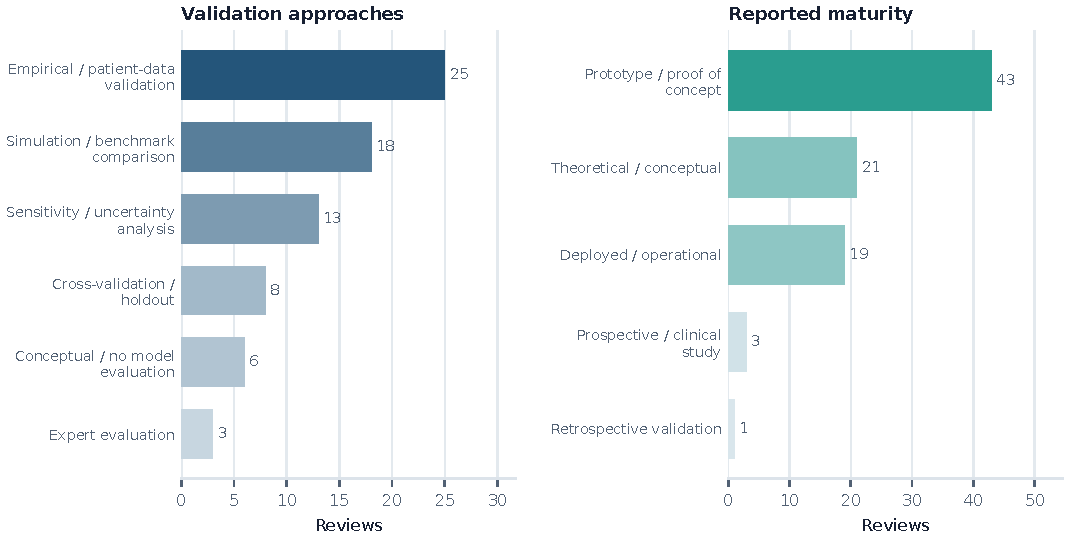
\includegraphics[width=0.94\textwidth]{fig4_validation_double_landscape.pdf}
    \caption{Validation approaches and reported maturity. Bars show non-mutually exclusive record-level mentions.}
    \label{fig:validation}
\end{figure*}

\subsection{Applications}

Applications spanned multiple clinical and research domains. Because reviews commonly addressed more than one domain or function, the application landscape is represented as a co-occurrence matrix rather than a forced single-label classification (Table~\ref{tab:applications}; Figure~\ref{fig:applications}).

\input{generated/tables/table5_applications}

\begin{figure*}[!tbp]
    \centering
    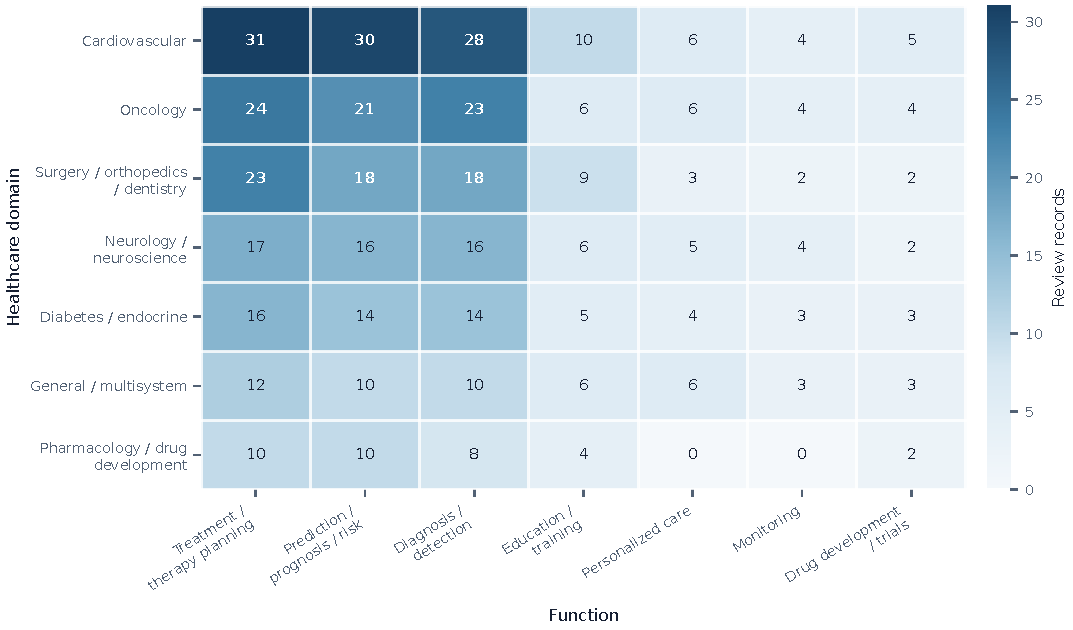
\includegraphics[width=0.94\textwidth]{fig5_applications_double_landscape.pdf}
    \caption{Application landscape. Cells show the number of review records in which a healthcare domain and function co-occurred.}
    \label{fig:applications}
\end{figure*}

\subsection{Barriers and future directions}

Cross-cutting limitations were classified into interoperability and standards; privacy, security, and governance; ethical, legal, and regulatory issues; computing and scalability; clinical adoption and workflow; data quality and availability; and validation, evidence, and reproducibility (Table~\ref{tab:barriers}; Figure~\ref{fig:barriers}). The corresponding reporting and implementation priorities are summarized in Table~\ref{tab:recommendations}.

\begin{figure}[H]
    \centering
    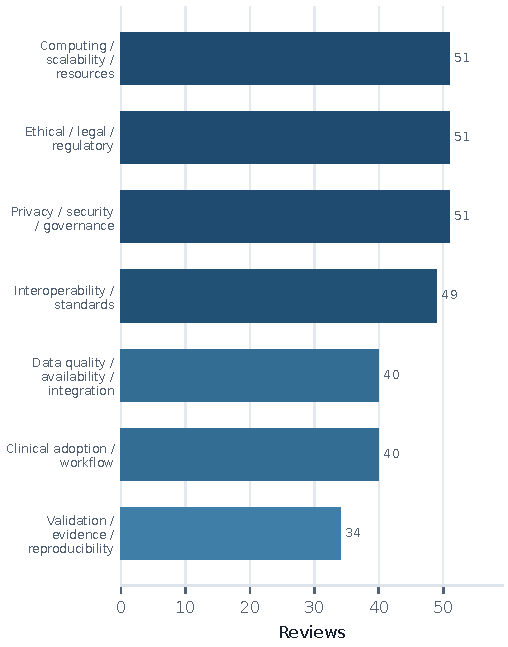
\includegraphics[width=\columnwidth]{fig6_barriers_single_portrait.pdf}
    \caption{Cross-cutting barriers. Bars show non-mutually exclusive record-level mentions.}
    \label{fig:barriers}
\end{figure}

\input{generated/tables/table6_barriers}
\begin{table*}[htbp]
\centering
\small
\caption{Future directions and recommendations derived from the extraction framework.}
\label{tab:recommendations}
\begin{tabularx}{\textwidth}{@{}>{\raggedright\arraybackslash}p{0.20\textwidth}YY@{}}
\toprule
\textbf{Recommendation} & \textbf{Priority} & \textbf{Evidence basis and suggested action} \\
\midrule
Standardize terminology & High & Report explicit criteria for digital model, digital shadow, digital twin, patient digital twin, virtual patient, and in silico patient. \\
Define maturity levels & High & Classify patient specificity, hierarchy, temporal updating, data coupling, feedback, validation, and clinical integration. \\
Strengthen validation & High & Require clear validation datasets, internal/external validation where relevant, and sensitivity or uncertainty analysis. \\
Build interoperable infrastructure & High & Report applicable FHIR, HL7, DICOM, OMOP, ontology, identifier, and governance mechanisms. \\
Provide reproducible supplements & High & Publish row-level extraction outputs, executable rules, data-quality checks, and plotting datasets. \\
Study workflow and governance & Medium & Evaluate clinician trust, liability, consent, bias, interpretability, equity, and implementation burden. \\
Move toward prospective evidence & High & Distinguish conceptual promise from retrospective validation, prospective studies, and deployed clinical workflows. \\
\bottomrule
\end{tabularx}
\end{table*}


\FloatBarrier

\section{Discussion}

\subsection{Principal findings}

The extracted literature supports a multidimensional framework for the digital patient spectrum. The most useful axes are the modeled biological scale, degree of patient specificity, temporal orientation, data-coupling mode, modeling approach, function, validation evidence, and maturity. A definition based only on the phrase \emph{digital twin} is too coarse for healthcare, where a static image-based simulation, an in silico trial cohort, and a continuously updated patient replica may be described with adjacent language.

The central translational gap is not lack of enthusiasm but lack of operational specificity. Reviews repeatedly describe personalized care, prediction, diagnosis, monitoring, and treatment planning, while fidelity metrics, validation datasets, uncertainty analysis, reproducibility, interoperability, governance, and workflow integration are reported unevenly. These gaps make it difficult to distinguish a conceptual prototype, research simulation, decision-support artifact, and operational patient twin.

\subsection{Implications}

Future work should prioritize a reporting and appraisal standard for digital patient reviews and primary models. At minimum, studies should report the physical referent, biological hierarchy, data sources, update frequency, coupling direction, model architecture, validation strategy, uncertainty handling, interoperability standards, governance assumptions, and maturity level. Such a standard would help separate useful analogies from clinically ready infrastructure.

The repository structure demonstrates a practical mechanism for that transparency: protocol and adjudication documents are versioned with the extraction workbook; classification rules are explicit; row-level derived data are inspectable; tables and figures are regenerated by one command; and the manuscript imports generated artifacts directly. This arrangement does not replace substantive team adjudication, but it makes every descriptive count auditable and refreshable as extraction evolves.

\subsection{Limitations}

This synthesis is descriptive and does not estimate pooled effects. The extraction workbook contains free-text, multi-label fields with heterogeneous specificity, and regular-expression classification cannot resolve all semantic ambiguity. Counts are therefore record-level signals rather than independent study effects. Some quality-appraisal and reproducibility fields remain incomplete. Title-level duplicate normalization does not substitute for final bibliographic deduplication. Finally, the PRISMA source counts require arithmetic reconciliation before submission, as documented automatically in the generated quality report.

\subsection{Future work}

The next revision should complete team adjudication, reconcile duplicate records and PRISMA counts, finalize author affiliations and declarations, connect reference-manager records to the LaTeX bibliography, and validate classification rules against a manually reviewed subset. The pipeline can then be rerun without changing the manuscript layout.

\section{Conclusion}

Digital patient research is conceptually active but infrastructurally immature. Progress toward clinically deployable patient digital twins will require clearer taxonomy, stronger and more transparent validation, interoperable data architecture, prospective workflow evidence, and governance models that address privacy, equity, accountability, and reproducibility.

\section{Data and code availability}

The public reproducibility repository is available at \url{https://github.com/aghcv/dtreview}. It contains the editable manuscript and supplementary protocol appendices, analysis code, classification rules, derived record-level classifications, generated tables and figures, and automated quality-control reports. The source extraction workbook and copyrighted full-text reports are not distributed through the public repository. A versioned archival release, persistent identifier, and the shareable adjudicated dataset should be deposited before publication, subject to author approval and applicable redistribution restrictions.

\section{Declarations}

\subsection{Author contributions}
\textit{To be completed and approved by all authors before submission.}

\subsection{Funding}
\textit{To be completed before submission.}

\subsection{Declaration of conflicting interests}
\textit{To be completed before submission.}

\subsection{Ethics approval}
This study synthesizes published review literature and does not involve new human-participant data. Any institution-specific statement should be confirmed before submission.


\clearpage
\section{Supplementary Appendix S1: Prespecified review protocol}
\label{app:protocol}

This editable appendix summarizes the methods specified in the prospectively registered PROSPERO protocol for \textit{Conceptual Clarification of Digital Patient Frameworks, Methodological Approaches, and Infrastructural Gaps: Evidence from a Systematic Meta-Review}. The review was scheduled to begin on 24 October 2025. Preliminary searches and piloting of study selection had been completed at registration; formal screening had started, whereas extraction, appraisal, and synthesis had not.

\subsection{Aim and review questions}

The primary aim was to synthesize how the digital-patient spectrum---digital twins, virtual patients, in silico patients, and synthetic patients---is conceptualized, constructed, validated, and operationalized in healthcare, and to identify methodological and infrastructural gaps that limit clinical translation. The six prespecified questions addressed:

\begin{enumerate}[label=\textbf{RQ\arabic*.},leftmargin=*]
    \item definitional boundaries, distinguishing features, classifications, and hierarchy levels across the digital-patient spectrum;
    \item model architectures, data pipelines, coupling, temporal orientation, computational approaches, infrastructure, and interoperability standards;
    \item validation methods, fidelity measures, reproducibility, generalizability, and trustworthiness;
    \item healthcare domains, functional roles, maturity, personalization, benefits, and limitations;
    \item ethical, legal, technical, data, interoperability, organizational, and infrastructural barriers; and
    \item research directions, validation and reporting standards, emerging technologies, and governance priorities needed for clinical readiness.
\end{enumerate}

\subsection{Information sources and search concepts}

The protocol specified Web of Science, PubMed, IEEE Xplore, and Google Scholar, supplemented by reference-list searching and searches of TechRxiv, arXiv, bioRxiv, engrXiv, and medRxiv. Database syntax was to be adapted while preserving three concept blocks:

\begin{enumerate}[leftmargin=*]
    \item \textbf{Digital-patient construct:} digital twin, patient digital twin, digital patient, virtual patient, in silico patient, synthetic patient, virtual sibling, patient-specific computational model, virtual physiological human, VPH, or surrogate model.
    \item \textbf{Health context:} patient, medicine, healthcare, surgery, treatment, pharmacology, oncology, clinical care, physiology, pathophysiology, biomechanics, imaging, genomics, precision medicine, personalized medicine, medical devices, quantitative medicine, or preventive medicine.
    \item \textbf{Review design:} systematic review, scoping review, meta-analysis, meta-review, review of reviews, umbrella review, or structured review.
\end{enumerate}

Searches were limited to English-language reports published from 2020 onward. The protocol scheduled the initial search for October 2025 and an update before final manuscript submission. Preprints were to be checked for subsequently published versions to avoid duplicate inclusion.

\subsection{Eligibility criteria}

Eligible reports were systematic, scoping, umbrella, meta-, or structured narrative reviews that explicitly examined at least one generic or patient-specific digital model applied to human health. Models could represent biological organization from subcellular, cellular, tissue, and organ levels through whole-body and in silico populations. Eligible reviews had to address conceptual framing, model construction, application, validation, methodological evaluation, or scalability.

Exclusions comprised primary studies without a structured review methodology; editorials, perspectives, commentaries, and abstracts without sufficient methods; non-English reports; animal-only, non-biological, or purely technical models without patient linkage; and digital twins limited to hospitals, logistics, infrastructure, communication systems, or devices without patient-level modeling. Behavioral or educational simulations without a physiological, biomechanical, or biological patient representation were outside scope.

\subsection{Selection, extraction, and appraisal}

The protocol specified independent title and abstract assessment by two reviewers in CADIMA, followed by adjudication under the procedure in Supplementary Appendix S2. A standardized, piloted extraction form was organized around the six review questions. One reviewer extracted each included report and a second reviewer checked the entry for accuracy.

The protocol prespecified review-type-appropriate methodological appraisal using AMSTAR~2 or SANRA and a domain-based CADIMA assessment of review-level bias and validity. Appraisal covered eligibility, search completeness, study selection, extraction reliability, appraisal of included evidence, synthesis, validation claims, generalizability, implementation, and sponsorship. Ratings were intended to contextualize the synthesis rather than determine eligibility automatically.

\subsection{Synthesis}

The planned synthesis was narrative and descriptive, supported by tabular summaries and conceptual maps. Prespecified comparisons included generic or archetype-based versus individual patient-specific models; static versus dynamic or continuously coupled models; and educational applications versus clinical decision support and personalized care. No quantitative pooling was anticipated.

\clearpage
\section{Supplementary Appendix S2: Screening inconsistency-resolution protocol}
\label{app:adjudication}

\subsection{Title and abstract screening}

Each record was evaluated independently by two reviewers using three core questions:

\begin{enumerate}[leftmargin=*]
    \item Is the report a review with structured methodology?
    \item Does it address a digital patient, digital twin, or an eligible adjacent construct?
    \item Is it focused on human health or healthcare?
\end{enumerate}

Permitted responses were Yes, Unclear, and No. A record was considered potentially eligible for full-text review when there was no agreed No on any core question. Uncertainty at this stage therefore favored retrieval of the full report.

\subsection{Classification and resolution of discrepancies}

CADIMA-flagged inconsistencies were divided according to whether they could change the inclusion decision.

\paragraph{Category A: no effect on eligibility.}
This category included records for which both reviewers recorded No on at least one criterion, reviewers identified different but independently sufficient exclusion criteria, or a Yes/Unclear discrepancy occurred while another criterion already had two No judgments. The coordinator verified the pattern and finalized the exclusion as the third reviewer.

\paragraph{Category B: possible effect on eligibility.}
This category included direct Yes/No conflicts and mixed response patterns that could determine whether the report advanced. The coordinator initiated record-specific discussion; both reviewers briefly restated their rationales and indicated inclusion or exclusion. If uncertainty remained, the report advanced. When consensus could not be reached, the coordinator made the final decision as the third reviewer.

\subsection{Documentation responsibilities}

The coordinator categorized each discrepancy, facilitated Category B discussions, acted as the third reviewer when required, and ensured that the final judgment and rationale were documented in CADIMA. Reviewers provided concise, evidence-based rationales and participated in discussion for eligibility-affecting conflicts. This procedure was intended to make adjudication consistent, auditable, and conservative at the screening stage.


\bibliographystyle{SageV}
\bibliography{references}

\end{document}
